\documentclass[11pt,a4paper]{article}
\usepackage{siunitx} % si eenheden
\usepackage{hyperref}					% maak PDF van de thesis navigeerbaar
\usepackage{url}
\usepackage[toc,acronym,xindy]{glossaries}%voor afkortingen
\usepackage{amsmath}
\usepackage[official]{eurosym} % om euro symbool te kunnen gebruiken
\usepackage{graphicx}
\usepackage{svg}
\usepackage[final]{pdfpages}
\usepackage[square,numbers]{natbib} 
\bibliographystyle{IEEEtran}
\usepackage{tabularx}  % betere tabellen
\usepackage[small,bf,hang]{caption} % verbetering captions
\captionsetup[table]{singlelinecheck=off} % caption van tabellen links uitlijnen
\usepackage{color, colortbl}
\definecolor{Gray}{gray}{0.9}

\usepackage{titlesec} 					% voor mooiere paragraph
\titleformat{\paragraph}
{\normalfont\normalsize\bfseries}{\theparagraph}{1em}{}
\titlespacing*{\paragraph}
{0pt}{3.25ex plus 1ex minus .2ex}{1.5ex plus .2ex} % nog steeds voor paragraph


% =========== BELANGRIJK VR IN HET VERSLAG: Tonen dat je hebt nagedacht over dimensionering componenten! ===========

% MFA: zet zoekpad voor figure
\graphicspath{{fig/}}
\usepackage{float}                      % De optie H voor de plaatsing van figuren op de plaats waar je ze invoegt. bvb. \begin{figure}[H]

\begin{document}
\title{Embedded systems 2\\
	\Huge Report Cosy Cafeteria
}
\author{Robin Van de Poel\and Arthur Van den Storme\and Tobias Cromheecke\and Thomas Feys}
\date{\today}
\maketitle
\newpage

\tableofcontents
\newpage

\section{Intro}
To improve the experience of the students in the cafeteria, an embedded system will be developed to gather a variety of data. This data will then be display to the students through an online medium such as a website. The main focus will be to gather information about the amount of people that are in the cafeteria. There are two main goals. The first goal is to display the estimated waiting time to get a meal to the students. Secondly the amount of available seats will be tracked and displayed to the students. Next to this some additional information will be gathered. The temperature, air-quality and sound level will be monitored to give the student a general idea about the conditions in the cafeteria. This way the student can gauge if the cafeteria is suitable to study in at a certain moment. An overview of the envisioned system is displayed in figure~\ref{fig:system}. All the developed hardware and software is displayed at: \url{https://github.com/thomasf10/cosy_cafeteria}.
\begin{figure}[H]
	\centering
	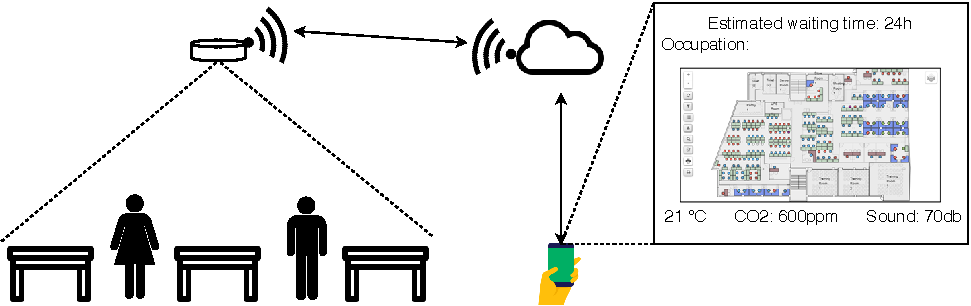
\includegraphics[width=1.0\linewidth]{situation.pdf}
	\caption{Situation sketch}
	\label{fig:system}
\end{figure}

\section{Specifications}
%Zoals we geleerd hebben in dit vak? eerst specs opstellen
%Hierbij moet de keuze's vermeld worden over:
% - Dimensions
% - Microcontroller 
\subsection{Functional specifications}
\begin{itemize}
	\item Monitor the available seats
	\item Monitor the queue to get a meal
	\item Display the data to the students
	\item Energy provision for 1 semester (4-5 months)
	\item Wireless coverage over the entire campus
	\item Measure new data every 10 minutes
	\item Send the data to the online medium every hour 
	\item If the data changes with a large amount (needs to be specified) update the online medium sooner
\end{itemize}

\subsection{Other technical specifications}
\begin{itemize}
	\item Enclosure: 10 x \SI{10}{\centi\meter}
	\item Easy deployment: the node must be easy to attach and detach from the sealing
	\item Must be easy to recharge (Wireless or via USB)
	\item Light weight: \SI{300}{\gram} (so it wont detach from the sealing)
\end{itemize}

\subsection{Non-technical specifications}
\begin{itemize}
	\item Cost: \euro{??}
	\item The data should be easy accessible to the students
\end{itemize}


\section{System architecture}
systeem wat uitleggen \dots
\textbf{!!EENS CHECKEN OF DE ARCHITECTUUR IN GROTE LIJNEN KLOPT}
An overview of the full system is displayed in figure~\ref{fig:architecture}.
\begin{figure}[H]
	\centering
	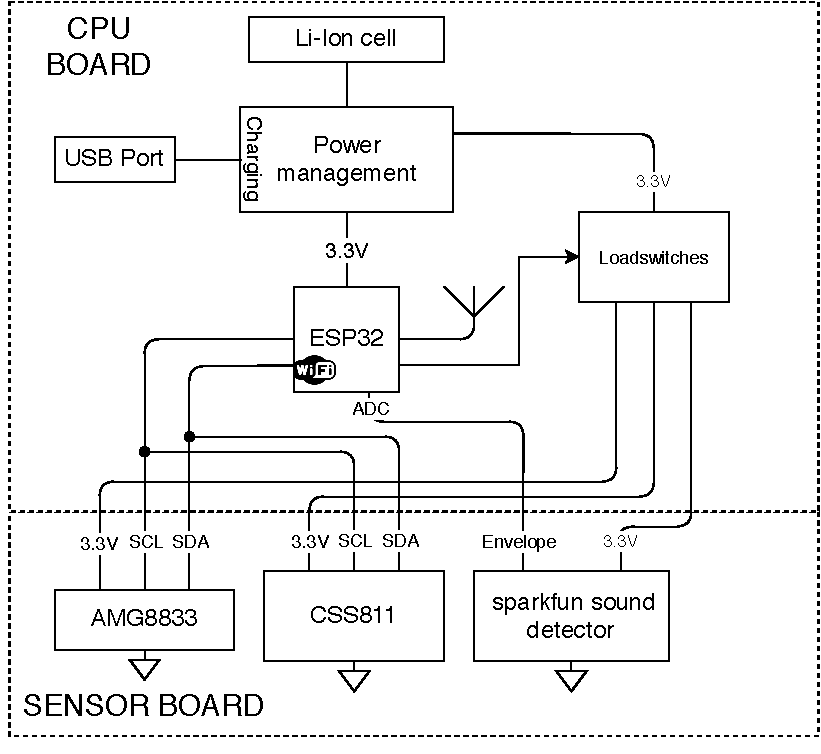
\includegraphics[width=1.0\linewidth]{architecture.pdf}
	\caption{System architecture}
	\label{fig:architecture}
\end{figure}
The developed system uses three sensors: 
\begin{itemize}
	\item AMG8833: IR grid sensor
	\item CSS811: air quality sensors
	\item Sparkfun sound detector: microphone
\end{itemize}
By incorporating these sensors in to the system, a variety of sensor data is gathered, namely: ambient temperature [\SI{}{\celsius}], $CO_2$-level [ppm], TVOC-level (total volatile organic compounds) [ppb] and sound level [db]. Next to this the AMG8833 captures the temperature af a two dimensional area in 8 by 8 pixels. 
\\ \\
The 'brain' of the system is an ESP32, this microcontroller has an integrated Wi-Fi module, which will be used to transmit the data. The gathered data is sent to a server, which stores the received data in a database. 
\\ \\
Alongside the reception of data from the ESP32, the server hosts a website which is used to display the data to the students. The website uses the pixel data to generate a heatmap of the cafeteria, this allows the students to see how many people are present in the cafeteria. Unfortunately one module cannot cover the entire cafeteria, to generate the heatmap. In order to do this, several modules have to be deployed in the cafeteria. In this project only one module will be constructed as a proof of concept. Next to the heatmap, the other sensor data is displayed on the website this includes: ambient temperature, $CO_2$-level, TVOC-level and the sound-level. Based on these parameters the students can gauge if the cafeteria is currently suitable as a study-location.


\section{Power management design}
This section explains the different trade-off's which were made in designing the power management part of the system. The first part in designing the power management is choosing a way to supply the circuit. In our case, the device needs to be deployed at the ceiling of a cafeteria. You can't just tap off the electricity cable at any point here, so our device will need a battery to supply the power. Our first aim was to supply the device as long as one semester. Another aspect was the ability to recharge the battery for environmental reasons. This excludes standard cell batteries that have a much lower energy density and are not rechargeable. Our choice was quickly made for the type of battery, namely a Lithium-Ion (Li-Ion) battery which will be discussed in section \ref{sec:liIon}.

\subsection{Lithium-Ion battery}\label{sec:liIon}
Lithium-Ion batteries are now a commonly used battery in consumer electronics. Li-Ion batteries is the most commonly used battery in phones, MP3 players and other portable equipment. The voltage of a single Li-Ion battery cell is usually fixed at 3.6 V or 3.7 V. We call this the nominal voltage. However, the actual voltage during use can vary from 2.4 V to 4.2 V. When the voltage drops below 2.4 V, the cell is discharged too deeply and damaged beyond repair. Therefore, a safety voltage of 3 V is often maintained. If the cell is discharged to this voltage, nothing is wrong. Charging a Li-Ion battery usually takes 3 hours. Don't be blinded by fast chargers for these batteries, practical tests have shown that it takes 3 hours until a battery is fully charged \cite{LiIon_ledscherp}. A few benefits of a Li-Ion battery are:
\begin{itemize}
	\item Very high energy density
	\item Minor self-discharge
	\item No memory effect
	\item High power, long service life
\end{itemize}
Some disadvantages are:
\begin{itemize}
	\item Relatively expensive to purchase
	\item Dangerous if used incorrectly, can explode/combust
	\item Need a protection circuit to not drop below the 2.4 V threshold value
	\item Charging and discharging process needed 
\end{itemize}
The most common Li-Ion battery is the 18650 cylindrical cell which is 18mm wide, 65mm long and the '0' stands for its cylindrical shape. Another common type of Lithium-Ion battery is the Lithium-Ion Polymer (Li-Po) battery.
%Li-Po's are:
%\begin{itemize}
%	\item Lighter
%	\item Faster recharge
%	\item Higher power: it's easy to produce batteries that can discharge 10C, 20C\footnote{\url{https://batteryuniversity.com/learn/article/what_is_the_c_rate}}.
%	\item Safer: less ability to explode/combust
%	\item Flexible: can bent (up to $90^\circ$) and deform + can be made in a variety of shapes
%	\item More expensive
%\end{itemize}
Li-Po's are preferred over standard Li-Ion batteries in application where weight reduction is important, fast charge opportunity is needed and which need a very high current during discharge time. Li-Po's are more used for drones (where lightweight is a requirement) and electric cars (fast charging requirement). Li-Po's are also less likely to combust or explode and are more expensive. Therefor a Li-Po would be overkill in our application \cite{LiIonVsLi-Po_Ovonic,LiIon_Wiki,Li-Po_Wiki}. 

\subsubsection{Selected battery}\label{sec:selected_battery}
The reason we chose a single cell Li-Ion battery was:
\begin{itemize}
	\item Voltage range: our microcontroller needs 3.3 V supply voltage, which is only a low dropout voltage of 0.4 V in comparison with the 3.7 V nominal voltage of a single cell Li-Ion battery. This results in less power dissipation in the voltage regulator. 
	\item Rechargeable: for environmental aspects
	\item High capacity: around 3000 mAh, to last a semester
\end{itemize}
The specifications of the chosen NCR18650B are:
\begin{itemize}
	\item Size/package: 18650
	\item Rated capacity: 3200 mAh
	\item Nominal voltage: 3.6 V
	\item Maximum voltage: 4.2 V
	\item Maximum charge current: 1625 mA
	\item Maximum discharge current: 6400 mA\footnote{Maximum discharge rate is 2C. This means discharging the battery capacity in 0.5 hours $\frac{3200 mAh}{0.5 h} = 6400 mA$ .} % https://batteryuniversity.com/learn/article/what_is_the_c_rate
	\item Maximum discharge voltage: 2.5 V
	\item Charge time: 4 hours
	\item No protection circuit
\end{itemize}
To charge the Li-Ion we had to include a charge circuit in our design. We found a high frequently used breakout board to charge a single cell Li-Ion battery via USB with battery protection \href{http://acoptex.com/project/9446/basics-project-082a-lithum-battery-charger-tp4056-at-acoptexcom/#sthash.3qJ5RSCy.AsMaJFMH.dpbs}{here}. Such a charge circuit would be perfect for our application. Due the reason we couldn't use a breakout board we had to integrate the components on one PCB. Unfortunately the components which were used on the breakout board were not available on the websites we're using to order components like Mouser, Digi-Key, Farnell, etc. After some research and a recommendation of a fellow student who had experience with battery charging applications in his master thesis, he advised to go for Texas Instruments IC's for charging Li-Ion batteries. The charger IC didn't had a protection circuit on it, so we also needed a circuit for this. Eventually we also went for a protection IC and voltage regulator of Texas Instruments. To protect the circuit for reverse polarity of the battery we also included an own-designed protection circuit which was first evaluated in LT Spice. All named components will be discussed in the following sections.

\subsection{Reverse polarity protection}
Reverse polarity protection is a nice feature to have te protect a circuit against polarity mismatches of the battery. For the design of this circuit we based us on a design found on the internet \href{http://kaktuscircuits.blogspot.com/2014/07/reverse-polarity-and-overvoltage.html}{here}. Before implementing this circuit in our design we first evaluated it's correct functioning using LT Spice in section \ref{sec:reverse_pol_prot_sim}.

\subsubsection{Simulation}\label{sec:reverse_pol_prot_sim}
Reverse polarity protection is simple done by including a P type MOSFET as shown in figure \ref{fig:reverse_polarity_protection_simulation}. Since the maximum voltage is limited to 4.2 V of the battery, there is no need for high drain-to-source voltage $V_{DS}$ requirements for the MOSFET. A suitable MOSFET was found \cite{bib:NTR2101P}. Normally there should be a zener diode placed between gate and source to protect the maximum gate-to-source voltage $V_{GS}$. Since the selected MOSFET's $V_{DS}$ = $V_{GS}$ = 8 V there is no need for a zener diode to clamp the voltage. 
% NTR2101P Spice model: https://www.digchip.com/application-notes/52/54566.php
\begin{figure}[H]
	\centering
	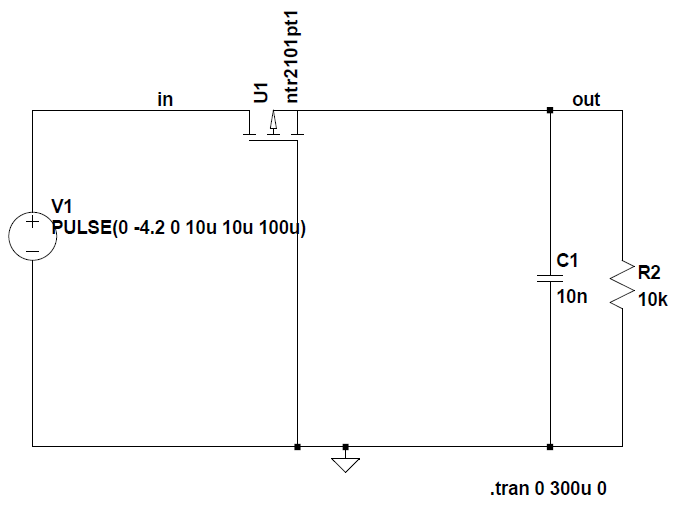
\includegraphics[width=0.8\linewidth]{reverse_polarity_protection_simulation.png}
	\caption{Simulation reverse polarity protection circuit}
	\label{fig:reverse_polarity_protection_simulation}
\end{figure}
Figure \ref{fig:Transient_response_negative_input_pulse} shows the transient response when applying a negative pulse at the input. As can be seen in the figure, the negative pulse doesn't come through the rest of the circuit. The voltage at the output is 0 V.
\begin{figure}[H]
	\centering
	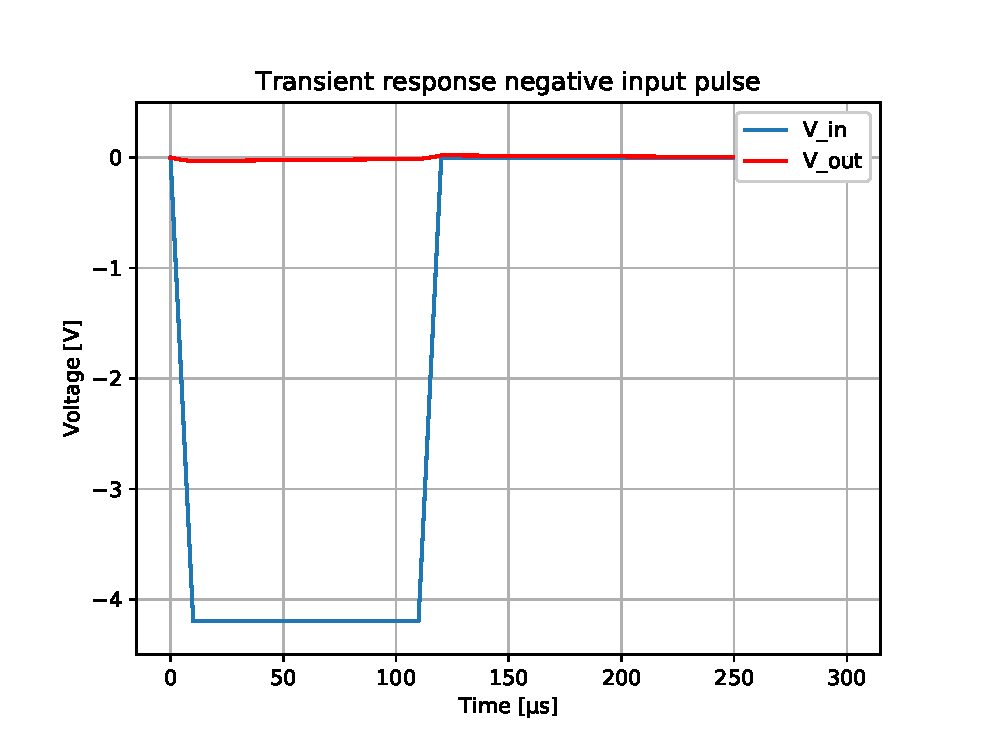
\includegraphics[width=0.8\linewidth]{Transient_response_negative_input_pulse.eps}
	\caption{Transient response negative input pulse}
	\label{fig:Transient_response_negative_input_pulse}
\end{figure}
When applying a positive pulse at the input, it can be seen in figure \ref{fig:Transient_response_positive_input_pulse} the output follows the input. We can evaluate the circuit works properly to protect against reverse polarity protection. Now it can be implemented in our design discussed in section \ref{fig:Transient_response_positive_input_pulse}.
\begin{figure}[H]
	\centering
	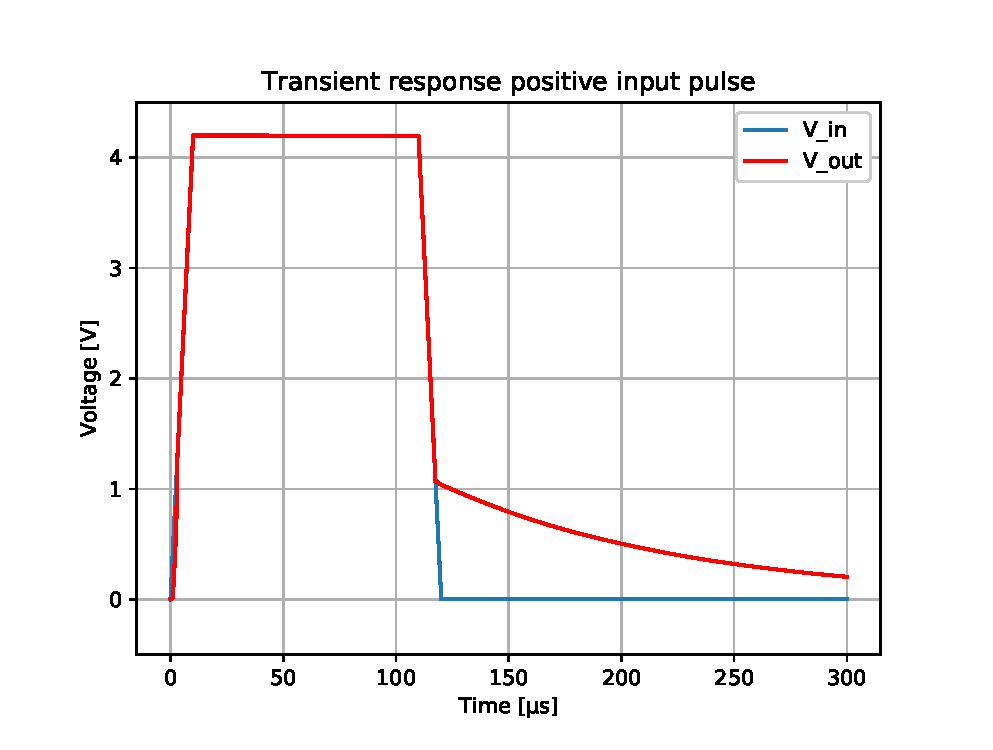
\includegraphics[width=0.8\linewidth]{Transient_response_positive_input_pulse.eps}
	\caption{Transient response positive input pulse}
	\label{fig:Transient_response_positive_input_pulse}
\end{figure}

\subsubsection{Implementation}\label{sec:reverse_pol_prot_implementation}
As a precaution we included two batteries in the first version of our design. This was done for debugging reasons: in case our real current consumption would be too high after trying every possibility to reduce it in software, we had an extra battery to meet our lifetime goal. It was possible to include an extra battery because the PCB dimensions were still lesser then 100 x 100 mm. JP1 is a footprint to solder a wire so we are able to measure the current using a current probe. When the battery is correct polarity of the battery is applied, +BATT is connected to VDD1.
\begin{figure}[H]
	\centering
	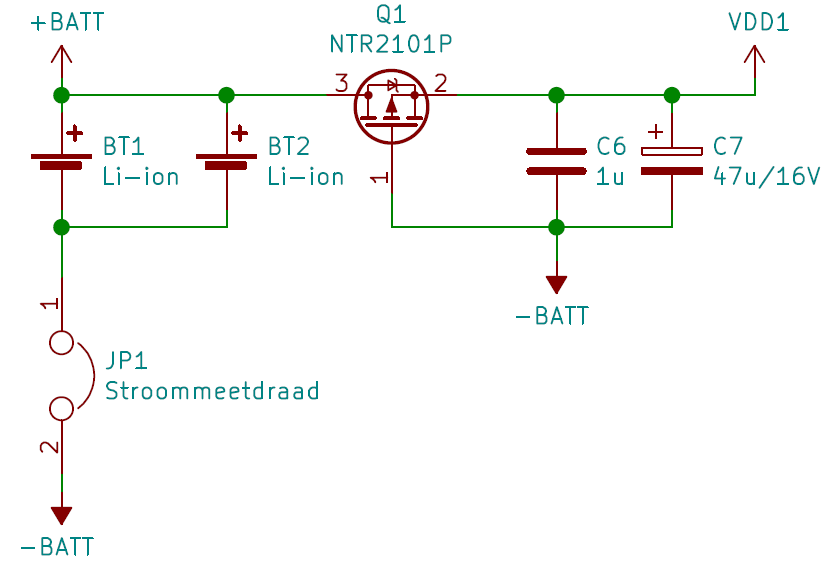
\includegraphics[width=0.8\linewidth]{reverse_polarity_protection.png}
	\caption{Reverse polarity protection circuit}
	\label{fig:reverse_polarity_protection}
\end{figure}

\subsection{Charging choice}
For charging you're free to choose at which voltage and current you charge. Eventually a Li-Ion charger IC will step down the voltage to the maximum 4.2 V for a cell. For charging you could design your own AC-DC converter, we went for the ability to charge the device using USB. Here for we rely on a power adapter which transforms 240 VAC to 5 VDC, or the ability to charge our device using a USB port on a computer. Figure \ref{fig:microUSBinput} shows the input connector micro USB type B with two decoupling capacitors $C_1$ and $C_2$. The charging voltage source is labeled as Vin.
\begin{figure}[H]
	\centering
	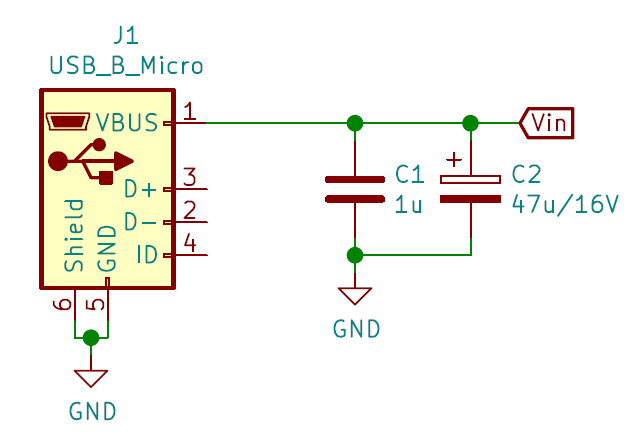
\includegraphics[width=0.8\linewidth]{microUSBinput.png}
	\caption{Micro USB type B input}
	\label{fig:microUSBinput}
\end{figure}

\subsection{Battery charging circuit}
We considerd many chips from different kind of manufacturers. As previously said a TP4056 IC charger is commonly used for single cell Li-Ion batteries, but it's not available on Digi-Key, Farnell, etc. Eventually we went with the BQ24075 IC from Texas Instruments. It's a great choice because it's made to charge a single cell Li-Ion battery, and it's perfectly fit to charge using a USB port. The IC operate from either a USB port or an AC adapter and support charge currents up to 1.5 A. The input voltage range with input overvoltage protection supports unregulated adapters. The USB input current limit accuracy and start up sequence allow the BQ24075 to meet USB-IF inrush current specifications\footnote{\url{http://www.testusb.com/inrush_issue.htm}}. Additionally, the input dynamic power management (VIN-DPM) prevents the charger from crashing incorrectly configured USB sources. An additional specification that was decisive in the choice of charger IC was the availability of 2 pins for status indication:
\begin{enumerate}
	\item \textbf{power good indication:} if the input voltage Vin is in specified range.
	\item \textbf{charge indication:} if the charger is charging (bright up LED) and when the charge cycle is complete (quench LED)
\end{enumerate}
Figure \ref{fig:bq24075_toegepast} shows the BQ24075 IC implemented in our design. A green LED D1 indicates the power good signal, and blue LED D2 indicates the charging stage. When no voltage is applied at the input Vin, the internal transistor Q1 is opened and Q2 is closed. Therefor VDD1 is connected to VDD2. During charge cycle both transistors Q1 and Q2 are closed allowing the battery to charge. The BQ24075 feature a SYSOFF input that allows the user to turn Q2 off and disconnect the battery from the OUT pin. This is useful for disconnecting the system load from the battery, factory programming where the battery is not installed or for host side impedance track fuel gauging, where the battery open circuit voltage level must be detected before the battery charges or discharges. We don't use this feature so we connect SYSOFF to GND to close Q2 for normal operating mode \cite{bib:BQ24075}. %Connect SYSOFF high to turn off the FET connecting the battery to the system output. When an adapter is connected, charging is also disabled. Connect SYSOFF low for normal operation. SYSOFF is internally pulled up to VBAT through a large resistor (approximately 5 M$\Omega$). Do not leave SYSOFF unconnected to ensure proper operation.
The other features of BQ24075 and schematic components will be discussed in sections \ref{sec:charging_phases} to \ref{sec:BQ24075_caps}.
\begin{figure}[H]
	\centering
	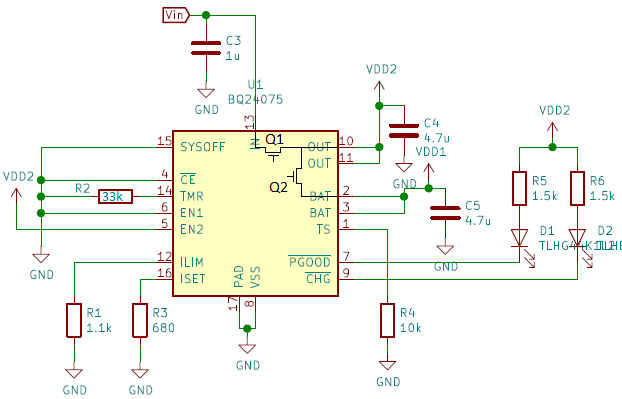
\includegraphics[width=0.9\linewidth]{bq24075_toegepast.png}
	\caption{Typical application circuit BQ24075}
	\label{fig:bq24075_toegepast}
\end{figure}

\subsubsection{Charging phases}\label{sec:charging_phases}
Set $\overline{CE}$ low to initiate battery charging. The battery is charged in three phases: 
\begin{enumerate}
	\item Conditioning pre-charge
	\item Constant current (CC) fast charge (current regulation) 
	\item Constant voltage (CV) tapering (voltage regulation)
\end{enumerate}
Figure \ref{fig:Charge _cycle} illustrates the three charging phases. In the pre-charge phase, the battery is charged at with the pre-charge current $I_{PRECHG}$. Once the battery voltage crosses the $V_{LOWV}$ threshold, the battery is charged with the fast-charge current $I_{CHG}$. As the battery voltage reaches $V_{BAT(REG)}$, the battery is held at a constant voltage of $V_{BAT(REG)}$ and the charge current tapers off as the battery approaches full charge. When the battery current reaches $I_{TERM}$, the CHG pin indicates charging done by going high-impedance.
\begin{figure}[H]
	\centering
	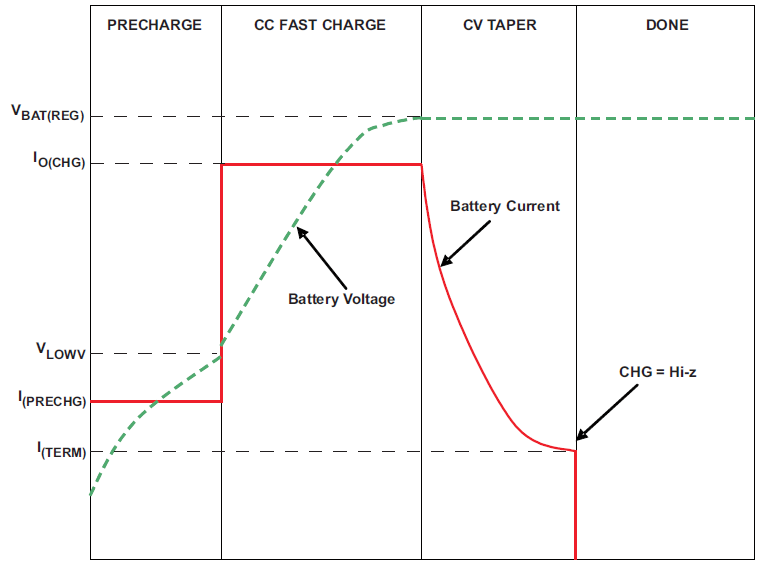
\includegraphics[width=1.0\linewidth]{Charge_cycle}
	\caption{Charge cycle \cite{bib:BQ24075}}
	\label{fig:Charge _cycle}
\end{figure}


\subsubsection{Set input current limit $I_{LIM}$}
The BQ24075 IC offers a fully compliant USB charger, meaning:
\begin{enumerate}
	\item Selectable 100 mA and 500 mA maximum input current
	\item 100 mA Maximum current limit ensures compliance to USB-IF standard
	\item Input-based dynamic power management (VINDPM) for protection against poor USB sources
\end{enumerate}
As shown in table \ref{table:USBmode}, EN1 and EN2 are used to configure the USB charge current.
\begin{table}[H]
	\caption{EN1/EN2 Settings \cite{bib:BQ24075}}
	\label{table:USBmode}
	\begin{tabular}{c|c|l}
		EN2 & EN1 & MAXIMUM INPUT CURRENT INTO IN PIN            				\\
		\hline
		0   & 0   & 100 mA. USB100 mode                          				\\
		0   & 1   & 500 mA. USB500 mode                          				\\
		1   & 0   & Set by an external resistor from ILIM to VSS (max. 1.5 A) 	\\
		1   & 1   & Standby (USB suspend mode)                  
	\end{tabular}
\end{table}
USB1.0 specifications allow devices to draw up to 500 mA from one port. USB operates at 5V, so that means a maximum of 2.5 watts. USB 2.0 has the same power limit. But later there were add-ons to the spec for battery charging, allowing up to 1.5A (7.5W) while data transfer is going on, and up to 5A if not. Few USB 2.0 devices can deliver that much power. Also note that the Micro USB connector is only rated to carry 2.1A (10.5W). USB 3.0 increases the power limit to 900mA (4.5W). The battery charging spec from USB 2.0 can optionally be supported \cite{USBpowers}. Since almost all USB chargers and ports are 2.0 and 3.0 nowadays, we can step up the current above 500 mA. The value of the input current limit $I_{LIM}$ is set by the resistor connected from the ILIM pin (pin 12) to VSS, and is given by \cite{bib:BQ24075}
\begin{equation}\label{equ:relationK_ILIM}
R_{ILIM} = \frac{K_{ILIM}}{I_{LIM}} \,,
\end{equation}
with 
\begin{equation}\label{equ:K_ILIM}
K_{ILIM} = 1610 A\Omega \,.
\end{equation}
The valid resistor range is 1.1 k$\Omega$ to 8 k$\Omega$. A value of 1.1 k$\Omega$ results in an input current limit 
\begin{equation}\label{equ:I_LIM}
I_{LIM} = \frac{1610 A\Omega}{1.1 k\Omega} = 1.46 A \,.
\end{equation}
The maximum input current limit 1.5 A is reached. \textbf{Caution:} make sure this current doesn't exceed the value of the maximum charge current of the battery, which is in our case within the permitted limit of 1625 mA (section \ref{sec:selected_battery}).


\subsubsection{Fast charge safety timer (TMR)}
TMR controls the pre-charge and fast-charge safety timers. Leave TMR open to set to default safety timers. Connect to VSS to disable safety timers. Connect a 18 k$\Omega$ to 72 k$\Omega$ resistor between TMR and VSS to program the timers a desired length. Reset the timers by toggling the CE pin, or by toggling EN1, EN2 pin to put the device in and out of USB suspend mode (EN1 = 1, EN2 = 1). The charge time of the battery is 4 hours (section \ref{sec:selected_battery}). We will calculate the TMR resistor $R_{TMR}$ to meet the desired charge time of 4 hours, using equation \cite{bib:BQ24075}
\begin{equation}
R_{TMR} = \frac{t_{MAXCHG}}{10 \cdot K_{TMR}} \,,
\end{equation}
with 
\begin{equation}
K_{TMR} = 48 \, s/k\Omega \,,
\end{equation}
\begin{equation}
t_{MAXCHG} = 4 hr \,.
\end{equation}
\begin{equation}
R_{TMR} = \frac{t_{MAXCHG}}{10 \cdot K_{TMR}} = \frac{4 \, hr \cdot 3600 \, s/hr}{10 \cdot 48 \, s/k\Omega} = 30 \, k\Omega
\end{equation}
Select a resistor value of 33 k$\Omega$, so it's E6-E12 compliant an to extend it charge time a little bit. Connect this resistor between TMR (pin 2) and VSS.


\subsubsection{Set fast charge current $I_{CHG}$}\label{sec:fastchargecurrent}
The value of fast-charge current $I_{CHG}$ is set by the resistor connected from the ISET pin to VSS, and is given by \cite{bib:BQ24075}
\begin{equation}\label{equ:relationK_ISET}
R_{ISET} = \frac{K_{ISET}}{I_{CHG}} \,,
\end{equation}
with
\begin{equation}\label{equ:K_ISET}
K_{ISET} = 890 A\Omega \,.
\end{equation}
The charge current limit is adjustable up to 1.5 A. The valid resistor range is 590 $\Omega$ to 8.9 k$\Omega$. If $I_{CHG}$ is programmed as greater than the input current limit $I_{LIM}$, the battery will charge at the rate of $I_{LIM}$ instead of $I_{CHG}$. In this case, the charger timers will be proportionately slowed down. The maximum charge current for the Panasonic NCR18650B battery is 1625 mA (section \ref{sec:selected_battery}). Set charge current to 1.3 A to have some margin for the battery lifetime and calculate the resistor value
\begin{equation}
R_{ISET} = \frac{890 A\Omega}{1.3 A} = 684.62 \Omega \approx 680 \Omega \,.
\end{equation}
Select the closest standard value (E6,E12,...), which for this case is 680 $\Omega$. Connect this resistor between ISET (pin 16) and VSS.
%The eventual charge current will be 
%\[ I_{CHG} = \frac{890 A\Omega}{680 \Omega} = 1.31 A \,. \]

%\subsubsection{Charge Current Translator}
%When the charger is enabled, internal circuits generate a current proportional to the charge current at the ISET input. The current out of $I_{SET}$ is 1/400 ($\pm$10\%) of the charge current. This current, when applied to the external charge current programming resistor, $R_{ISET}$, generates an analog voltage that can be monitored by an external host to calculate the current sourced from BAT.
%\[ V_{ISET} = \frac{I_{CHG}}{400} R_{ISET} \]


\subsubsection{TS function}
The TS-pin is the external NTC thermistor input. Connect the TS input to the NTC thermistor in the battery pack. TS monitors a 10 k$\Omega$ NTC thermistor. For applications that do not use the TS function, connect a 10 k$\Omega$ fixed resistor from TS to VSS to maintain a valid voltage level on TS.


\subsubsection{Selecting IN-, OUT-, and BAT-pin capacitors}\label{sec:BQ24075_caps}
In most applications, all that is needed is a high-frequency decoupling capacitor (ceramic) on the power pin, input, output and battery pins. Using the values shown on figure \ref{fig:bq24075_toegepast} (these are taken from the typical application circuit in \cite{bib:BQ24075}) is recommended. After evaluation of these voltage signals with real system operational conditions, one can determine if capacitance values can be adjusted toward the minimum recommended values (DC load application) or higher values for fast high amplitude pulsed load applications. Note if designed high input voltage sources (bad/wrong adaptors), the capacitor needs to be rated appropriately. Ceramic capacitors are tested to 2x their rated values so a 16-V capacitor may be adequate for a 30-V transient (verify tested rating with capacitor manufacturer).



\subsection{Battery protection circuit}\label{sec:bat_prot_circuit}
Due the battery we selected doesn't has an integrated protection circuit, we also needed to consider a battery protection circuit in our design. As discussed in section \ref{sec:liIon} it could lead to battery defect when the voltage of the battery drops below 2.4 V threshold value. A Li-Ion is also likely to explode/combust when charging too high in voltage or current. Therefor a protection circuit is always needed. We went for the BQ29700 which is a battery cell protection IC that provides an accurate monitor and trigger threshold for overcurrent protection during high discharge/charge current operation or battery overcharge conditions. The BQ29700 provides the protection functions for Li-Ion/Li-Po cells, and monitors across the external power FETs for protection due to high charge or discharge currents. Figure \ref{fig:bq29700_principeschema} shows a typical application circuit of the BQ29700 IC. In normal mode FETs Charge FET (CHG) and Discharge FET (DSG) are closed, however in one of the following conditions the FETs will open to stop the current flow from/to the battery:
%The system is operating in NORMAL mode when the battery voltage range is between the over-discharge detection threshold (VUVP) and the overcharge detection threshold (VOVP), and the V– pin voltage is within the range for charge overcurrent threshold (VOCC) to over-discharge current threshold (VOCD) when measured with respect to VSS. If these conditions are satisfied, the device turns ON the drive for COUT and DOUT FET control.
\begin{enumerate}
	\item \textbf{Overcharge detection (OVP):} When the cell exceeds the overcharge detection threshold voltage $V_{OVP}$ during charge, the safety circuit will interrupt the flow of current into the cell.% by opening CHG.
	When the overcharge voltage is exceeded, a delay of up to $t_{OVP}$ will occur before the FETs open the circuit.
	\item \textbf{Over-discharge detection (UVP):} When the cell exceeds the over-discharge detection threshold voltage $V_{UVP}$ during discharge, the safety circuit will interrupt the flow of current out of the cell.% by opening DSG. 
	When the over-discharge voltage is reached, a delay $t_{UVP}$ will occur before the FETs open the circuit.
	\item \textbf{Charge overcurrent detection (OCC):} When the pack output current the charge overcurrent detection threshold voltage $V_{OCC}$ during charge, the safety circuit will interrupt the flow of current out of the pack. When the charge overcurrent threshold voltage is exceeded, a delay of up to $t_{OCC}$ will occur before the FETs open the circuit.
	\item \textbf{Discharge overcurrent detection (OCD):} When the pack output current the discharge overcurrent detection threshold voltage $V_{OCD}$ during discharge, the safety circuit will interrupt the flow of current out of the pack. When the discharge overcurrent threshold voltage is exceeded, a delay of up to $t_{OCD}$ will occur before the FETs open the circuit.
	\item \textbf{Load short-circuit detection (SCD):} Similar to overcurrent threshold values, except a short circuit will result in a much higher current, thus a higher sense voltage. The short-circuit detection threshold voltage is indicated as $V_{SCD}$ with delay $t_{SCD}$.
\end{enumerate}
Specifications of the BQ29700 IC are \cite{bib:BQ29700}:
\begin{itemize}
	\item $V_{OVP}$ = 4.275 V
	\item $t_{OVP}$ = 1.25 s
	\item $V_{UVP}$ = 2.8 V
	\item $t_{UVP}$ = 144 ms
	\item $V_{OCC}$ = –0.1 V
	\item $t_{OCC}$ = 8 ms
	\item $V_{OCD}$ = 0.1 V
	\item $t_{OCD}$ = 20 ms
	\item $V_{SCD}$ = 0.5 V
	\item $t_{SCD}$ = 250 $\mu s$
\end{itemize}
\begin{figure}[H]
	\centering
	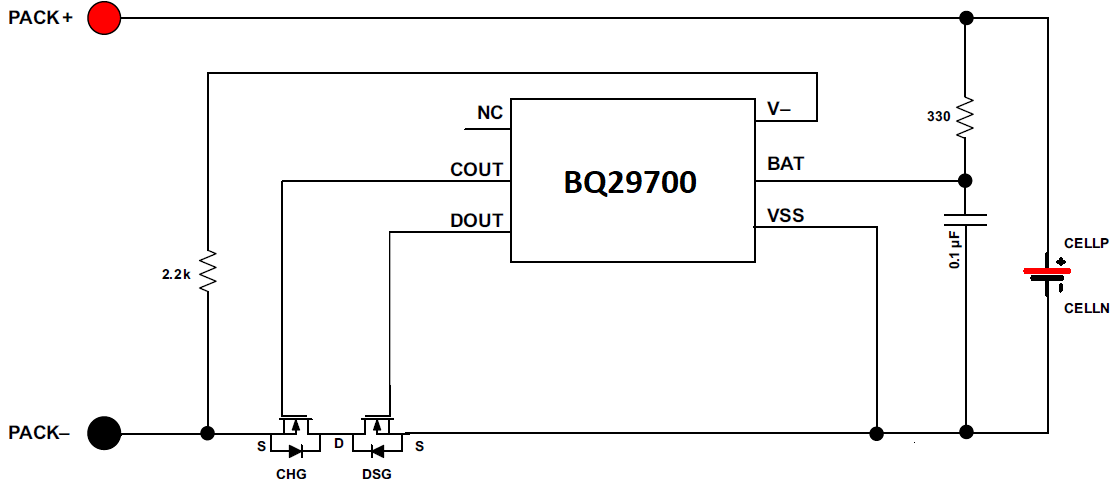
\includegraphics[width=0.9\linewidth]{bq29700_principeschema.png}
	\caption{Typical application circuit BQ29700 \cite{bib:BQ29700}}
	\label{fig:bq29700_principeschema}
\end{figure}

\subsubsection{Dimensioning}
Figure \ref{fig:bq29700_toegepast} shows the implemented BQ29700 IC in our design. An RC filter is required on the BAT-pin for noise, and enables the device to operate during sharp negative transients. The 330 $\Omega$ resistor also limits the current during a reverse connection on the system. TI recommends placing a high impedance 5 M$\Omega$ across the gate source of each external FET to deplete any charge on the gate-source capacitance. The voltage sense node $V_-$ is a sense node used for measuring several fault detection conditions, such as overcurrent charging or
overcurrent discharging configured as Vds sensing for protection. This input, in conjunction with VSS, forms the differential measurement for the stated fault detection conditions. A 2.2 k$\Omega$ resistor is connected between this input pin and Pack– terminal of the system in the application.
\\ \\
\textbf{FET Selection:} These should be MOSFETs who operate at relativly low voltages (2.8-4.2V battery cell) and that can handle a current of 1.3 A for charging (section \ref{sec:fastchargecurrent}). Due the current is measured by the voltage drop across the FETs, it's $R_{DSON}$ value is also an important value by choosing the right MOSFET. We chose FDS9926A, as it's a dual N-channel MOSFET IC. So both charge and discharge MOSFETs are integrated in one IC. Each FET's $R_{DSON}$ = 35 m$\Omega$ at Tj = 25 $^\circ$C and Vgs = 3.7 V (nominal battery voltage) \cite{bib:FDS9926A}. Because both discharge and charge overcurrent detection levels are the same (100 mV), the discharge and charge current are limited to approximately $\frac{100 mV}{2 \cdot 35m\Omega}$ = 1.43 A \cite{bib:BQ29700, bib:FDS9926A}.
\begin{figure}[H]
	\centering
	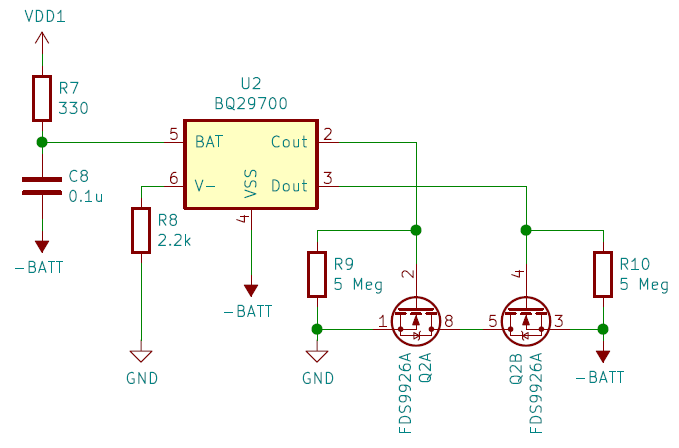
\includegraphics[width=0.9\linewidth]{bq29700_toegepast.png}
	\caption{BQ29700 applied schematic}  %% AANPASSEN!!!
	\label{fig:bq29700_toegepast}
\end{figure}


\subsection{Voltage regulator}
A few important points to consider when selecting the voltage regulator are:
\begin{enumerate}
	\item Low quiescent current\footnote{Current which is flowing though the converter when no load is applied.} $I_Q$ to reduce power losses for extended battery lifetime.
	\item Low dropout voltage\footnote{The Dropout Voltage of a regulator is the amount of voltage that a regulator needs to be fed above its rated output voltage to maintain the output voltage.} $V_{DO}$ due to the small difference between the 3.7 V nominal voltage of the battery and 3.3 V supply voltage for the ESP32 microcontroller.
	\item At least 500 mA maximum output current $I_{OUT,MAX}$ needed for ESP32 spikes \cite{bib:ESP32-SOLO-1}.
\end{enumerate}
In low power applications a linear regulator is preferred over a switching regulator due the fact switching converters are inefficient at very low loads, and power dissipation in the linear regulator is also low when combined with a low dropout voltage ($P^{\downarrow\downarrow} = U_{DO}^\downarrow\cdot I^\downarrow$). Linear regulators also have much lower quiescent currents in comparison to switching regulators \cite{LDOvsSwitch:1, LDOvsSwitch:2}

\subsubsection{Selected regulator}
As shown in figure \ref{fig:TLV75533_toegepast} we chose TLV75533 from Texas Instruments, with following parameters:
\begin{itemize}
	\item $I_Q$ = 25 $\mu$A (Typical)
	\item $V_{DO}$ = 150-238 mV (@ $I_{OUT}$ = 500 mA and $V_{OUT}$ = 3.3 V)
	\item $I_{OUT,MAX}$ = 500 mA
\end{itemize}
This device features an internal soft-start to lower inrush current, thus providing a controlled voltage to the load and minimizing the input voltage drop during start up. When shutdown, the device actively pulls down the output to quickly discharge the outputs and ensure a known start-up state. For protection reasons the TLV75533 has an integrated thermal shutdown, current limit, and undervoltage lockout (UVLO). 
\\ \\
Additionally, the TLV75533 has an enable functionality to minimize standby power. Unfortunately we can't use this function because the LDO supplies the microcontroller (these control signals to drive the enable pin should originate from the microcontroller). Therefor the enable pin is connected to the input pin to enable when an input voltage is supplied. 
\\ \\
The TLV75533 requires an output capacitance of 0.47-200 $\mu$F for stability. Use X5R- and X7R-type ceramic capacitors because these capacitors have minimal variation in capacitance value and equivalent series resistance (ESR) over temperature. Place a 1 $\mu$F or greater capacitor on the input pin of the LDO. Some input supplies have a high impedance. Placing a capacitor on the input supply reduces the input impedance \cite{bib:TLV755P}.
\begin{figure}[H]
	\centering
	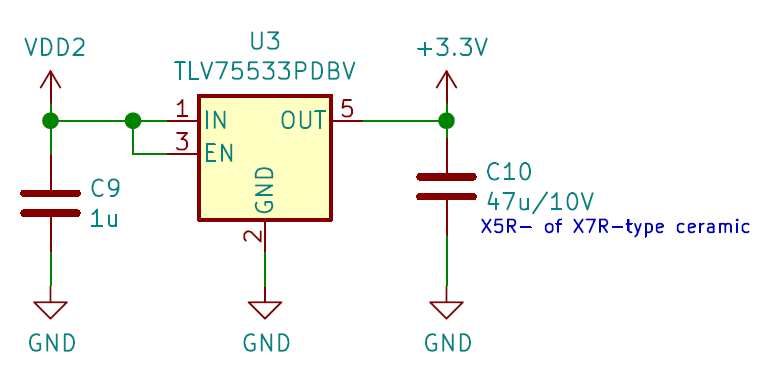
\includegraphics[width=0.9\linewidth]{TLV75533_toegepast.png}
	\caption{TLV75533 applied schematic}
	\label{fig:TLV75533_toegepast}
\end{figure}

\subsection{Load switches}
To reduce power even further you can disable the sensors by shutting off their supply voltage if they're not needed. This can be done by load switches or relays. A load switch is a small electronic switch used to configure and manage power distribution. You can make a load switch with discrete components, but there are significant advantages to using a fully integrated IC load switch \cite{loadSwitch}:
\begin{enumerate}
	\item \textbf{Saves space:} A key advantage of the integrated device over discrete load switches is the small footprint. 
	\item \textbf{Simpler design:} No discrete design time is required. Just buy the integrated chip and design it in to get all benefits and features.
\end{enumerate}
Load witches also has several advantages over relays \cite{loadSwitch}:
\begin{enumerate}
	\item \textbf{Quick output discharge:} An internal resistance in the form of a conducting MOSFET is connected across the load. It serves to discharge to the output capacitor quickly when the enable input goes low.
	\item \textbf{Reverse-current blocking:} Some IC load switches implement a feature that blocks any reverse current. When the enable input goes low to turn off the switch, the reverse current block circuit is enabled thereby reducing any potential reverse current from output back to input to a very low level.
	\item \textbf{Saves power:} Using load switches to manage the power output of the supply minimizes power consumption, saves energy, and provides for longer battery life in portable applications. In its off state, the IC draws minimal quiescent current.
	\item \textbf{Manages inrush current:} This feature prevents input voltage droop that may transpire when the switch is first turned on. This is the result of a high inrush current that occurs when charging the output capacitor. Most load switches provide a controlled ramp up of the output voltage as it charges the output capacitor.
	\item \textbf{Implements sequencing:} Load switches let you implement the sequencing of loads during a turn-on or turn-off operation. Some designs with processors, FPGAs, and other chips require that different supply voltages be applied or disconnected in a specific order. Multiple load switches for each supply that are operated by the related embedded controller for timing meet this need. Certain load switches also feature an output signal that indicates when the output is fully turned on. This signal can be used in sequencing operations with other load switches in the system.
\end{enumerate}

\subsubsection{Selected load switches}
The TPS22919 device is a small, single channel load switch with controlled slew rate. The device contains an N-channel MOSFET that can operate over an input voltage range of 1.6 V to 5.5 V and can support a maximum continuous current of 1.5 A. A few important specifications are \cite{bib:TPS22919}:
\begin{itemize}
	\item Input operating voltage range $V_{IN}$: 1.6 V to 5.5 V
	\item Maximum output current $I_{OUT,MAX}$ = 1.5 A
	\item Low power consumption:
	\begin{itemize}
		\item ON-state $I_Q$ = 8 $\mu$A (typical)
		\item OFF-state $I_{SD}$ = 2 nA (typical)
	\end{itemize}
	\item On-Resistance $R_{ON}$: 89 m$\Omega$ (typical) @ $V_{IN}$ = 5 V
\end{itemize}
The switch ON state is controlled by a digital input that is capable of interfacing directly with low-voltage control signals. When power is first applied, a Smart Pull Down is used to keep the ON pin from floating until system sequencing is complete. Once the pin is deliberately driven High ($> V_{IH}$), the Smart Pull Down will be disconnected to prevent unnecessary power loss. The TPS22919 load switch is also self-protected, meaning that it will protect itself from short circuit events on the output of the device. It also has thermal shutdown to prevent any damage from overheating.
\\ \\
Figure \ref{fig:TPS22919_toegepast} shows the application of TPS22919 for our 3 sensors. The resistor between VOUT and QOD pin is a quick discharge resistor to discharge the output capacitor when the enable pin goes low. For both in- and output capacitors, and the resistor, we used the recommended value as given in the datasheet \cite{bib:TPS22919}.
\begin{figure}[H]
	\centering
	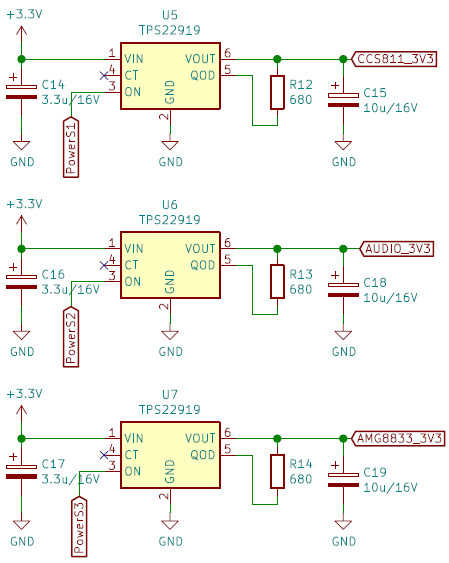
\includegraphics[width=0.8\linewidth]{TPS22919_toegepast.png}
	\caption{TPS22919 applied schematic}
	\label{fig:TPS22919_toegepast}
\end{figure}


\section{Microcontroller}
\begin{figure}[H]
	\centering
	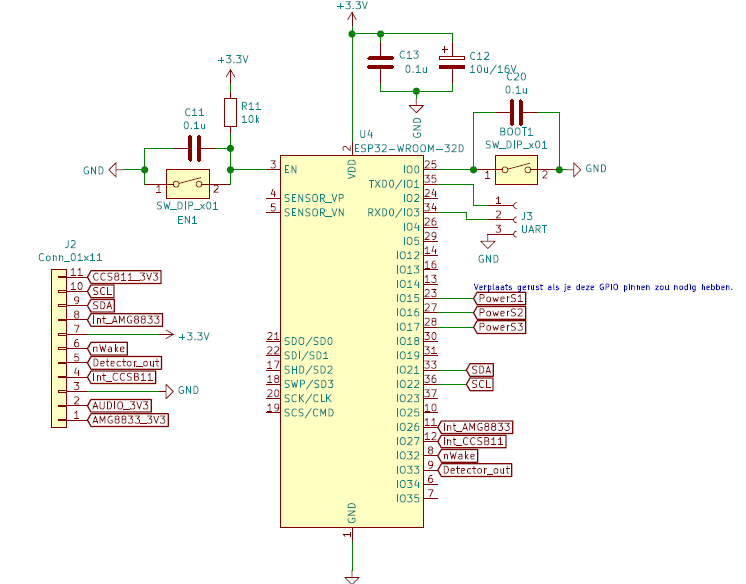
\includegraphics[width=1.0\linewidth]{ESP32_toegepast.png}
	\caption{ESP32 applied schematic}
	\label{fig:ESP32_toegepast}
\end{figure}


\section{Sensorboard}
\subsection{Design considerations}
For the sensorboard design, we have agreed to go for a seperated board from the main board. This gave us the possibillity to design it more freely. For the design, we have choosen to go for a two sided printed circuit board or PCB. All sensors will be put on the top side of the board for it will be plugged onto the CPU board. Then, we looked what sensors are needed for the design. The impulses that needed to be sense are the sound level, air quality, temperature and the the presences of people.
With the known knowledge about sensors for these impulses, we have choosen to go for the following sensors:

\begin{itemize}
	\item AMG8833 IR-sensor
	\item CCS811 air quality sensor
	\item BOB-12758 microphone breakout board
\end{itemize}
The main focus for the sensor board was how can we make it so low power as possible. As already mentiond above we have foreseen load switches to cut off the power when the system will be non active for a longer period of time. Beside the load switches, we have looked at the sensors to optimize the measuring sequence.

\subsection{AMG8833 IR-sensor}
To detect human presence, we have decided to use infrared. The human body produces quite some body heat that will be emited. The AMG8833  is an 8x8-pixel IR- sensor what will give us a heat map according to the pixel value. This will help us when determing how many people are presence in a certain area. For example we can determine not only single persons but also a group of persons as a row. 
\\ \\
One of the considarations we needed to investigate is the effect of distance, ambient temperature and the field of view of the sensor. This sensor has a total angle view of 60 ° for the horizontal and vertical axis of the pixelgrid. Depending on the height the area that the sensor cover will be different. The area will increase related to the heigth the sensor is installed. Not only the field of view will be influence by the height but also the result of the measurements. The further the heat source is away from the sensor, the less the sensor will detects the heat from it. 
\\ \\
The sensor operates in the temperature range of 0 °C up to 50 °C for the full humidity range between the 15 \%RH and up to about 85 \%RH. Higer temperatures can be handles if the huimidity stays below a certain value. This is illustatrated below. Because, the system will be applied in the cafeteria, this should not be a problem. An other aspect about the ambient temperature is the difference in measuring the heat of a person and that of the surroundings. This will be tested and will be implemented in the software. 
\\ \\
All communication to and from the sensor is done over I²C. In addition to hte I²C-communicatie there is a AD-select input to set the I²C-address, you can set to 0x58 or 0x59. There is also an interrupt output if you want to work with interrupts.
\\ \\
The last important aspect for this sensor is the power consumption. We can find in its documentation that it has a typical current of 4.5 mA in normal operation mode. When the sensor is brought to sleep the current will drop to 0.2 mA. Our goal is to wake the sensor from sleep and when we have the measurement put in him as fast as possible back to sleep.


\subsection{CCS811 air quality sensor}
For the air quality in the cafeterie, we have choosen to go for the CCS811 air quality sensor. The CCS811 is an ultra low power gas sensor with propable algortime system for detecting gasses. It has  the ability for sensing TVOC and an equivalent $CO_{2}$ concentration.This sensor has different measure modes that can help to make the application more flexible but also suitable for mobile equipment and battery powered systems. All settings and communication to the sensor is again done with I²C. The I²C-addresses are 0x5A and 0x5B, dependinng on the ADDR-pin. Beside I²C-communication there are some other signals that can control/monitor the sensor. 
\begin{itemize}
	\item There is a ADDR-pin for setting the I²C-address to 0x5A or 0x5B
	\item The nINT-pin is a active low pin, that generates interrupts depending on his settings. This pin can generate interrupts when a measurement is available or when the equivalent $CO_{2}$ is above or under a certain value. Tthis is an value that is best been buffered for monitoring with a GPIO-pin.
	\item The nReset-pin is not only a reset pin as an input but also can be monitered to detect a software reset.This can also be an input. If this pin is been pulled low you can reset the sensor.
	\item Finally, we have the nWake-pin what is also an active low pin. This pin can be used to put the sensor into sleep just by pulling the pin low.
\end{itemize}
The following modes are possible:
\begin{itemize}
	\item Idle: sensor does not perform a measurement, low current mode
	\item Mode 1: a measurement after every second, constant power mode
	\item Mode 2:  a measurement after every 10 seconds, Pulse heating mode
	\item Mode 3:  a measurement after every 60 seconds, Low power pulse heating mode
	\item Mode 4: a measurement after every 250 millisecond, constant power mode
\end{itemize}
The Idle-mode has a second purpose when switching from one mode to another. There is a requirement when changing the mode fom one with a higher sample rate a lower one the sensor must be put in idle for at least 10 minutes. This is not interesting in our purpose if we want to handle more flexible the sample rate. When changing the mode from a lower to a higher sample rate this is not needed. In our application, we have choosen to search for one mode to operate in and always placing the sensor back to sleep after the measurement has been read out.
\\ \\
In the documentation, we could find the average current for a pulse cycle is $0.7 mA$ with a power supply of $1.8 V$. If we put this in a calculation, we get the following result:
\\ \\
$P= U \cdot I=1.8 V \cdot 0.7 mA = 1.26 mW$
\\ \\
What is the power consumption of mode 3. And, if we compare it with the power consumption of mode 2 we can find:
\\ \\
$\frac{P_{pulse mode}}{P_{low pulse mode}}= \frac{7 mW}{1.26 mW}= 5.556$
\\ \\
This is not aspected, You can perform 6 times the measurements with a lower power consumption.
\\ \\
If we now perform the same comparison with mode 1 \& 4, we get the following result:
\\ \\
$\frac{P_{constant power}} {P_{low pulse power}}= \frac{46mW}{1.2 mW}= 38.333$
\\ \\
The power consumption of the constant power modes  is only a factor 38,333 bigger then it is in the low pulse power mode. While the amount of measurement is much higher in the constant power mode. This is something that could make our application more low power. This will be investigated by studying the measure behavior of the sensor. To make it possible that we could use he interrupt functionality of the CSS811, we have foreseen a buffer with an operationale amplifier for the nINT-signal.  This is foreseen in the prototype and if not implemented in the final design, this can be not implemented. The nINT is not an essentiel connection for the CSS811 to work properly.


\subsection{BOB-12758 microphone breakout board}
We have informed us by colleague students who had  use a microphone module in the first semester. One group came with a breakout board with a microphone and a triple op erational amplifier circuit. The proposed break out board could do several things, one of them was peak detection. For our application,there is only the need to check the average sound level, so we only needed a microphone and one operational amplifier. 
\\ \\
Because we wanted to have the average sound level, we decided to place a detector behind the opamp. The second reason to use the detector is that the ESP32 can sample up to about 27 ksps. By just looking at the sample rate, it is clear that the ADC is not high enough to fullfill the Nyquist theorema. 
\\ \\
The detector needs time to come from the low level to the sound level. Finding the best value of $\tau$ will be one of the investigations. This will be determine along with the test of the other sensors. For the time the supply needs to be apply must be about 10 times $\tau$. We know from the theory that after 5 $\tau$, 97\% of the applied voltage is reach. The extra 5 $\tau$ is chosen for two reasons. Firstly to compesate the rectified signal by the detector and secondly to have a stable value of the average sound level.

\subsection{Board design}
When designing the board, I have started from the basic schematics of the provided break out boards of the sensor boards. For the microphone sensorboard as mentioned we needed to design a detector circuit. We have choosen to go a simple detector with a diode followed by a RC circuit. During documentating the circuit it was noticed that the audiosignal of the breakout board is superpositioned onto a DC-voltage that is the half of the supply voltage. In the prototype of the board, this was not taken into consideration. This can be solved in different ways not only by hardware but also by software. If we want to solve this with hardware without loosing information, we can just put several diodes in serie untill we come to a sum of forward voltage that is the half of our voltage supply. The power supply is $3.3 V$. \\
$V_{Audio DC} = \frac{V_{cc}}{2}= \frac{3.3V}{2} = 1.65V$\\
This $1.65 V$ can approximatly be obtained by placing 2 schottkey diode with a $V_{f}=0.45 V$ and a normal diode with $V_{f} = 0.7 V$ in serie.\\
$V_{f total} = 2\cdot V_{f schottkey} + V_{f normal diode} = 1.6 V$\\
This will almost eliminate all the DC voltge in the audiosignal. \\
A better approach of the problem would be to solve this with software. To solve, this we can solve this by first nowing the ADC value at the DC value after the detector when there is no sound. The DC voltage after the detector will be $0.45 V$ less then before because of the schottkey diode.\\
$V_{DC offset} = \frac{V_{cc}}{2}-V_{f schottkey}= \frac{3.3 V}{2}- 0.45 V = 1.2 V$
We have a reference value of $1.2 V$ that is equal to no sound. The maximum audio voltage level would be $2.85 V$. What sound level this would be is unknow to us we could had calibrated the sensor value so we could do a convertion from voltage value to decibels. The DC-offset has a positieve effect on the detection of the sound level. Because the value is above the forward voltage of the diode we do not loose information on the amplitude. But as mentioned, we need to do a convertion depending on the two found boundries ( $1.2 V$ and $2.85 V$). It would also be interesting to calibrate the output between these boundries. This could not been done with the current corona situation. We did not have a microphone breakout board at our disposal.

To determin the optimal value for the resistor and the capacitor, we would wait to look at the other response time of the other two sensors. We have taken a initial value of 1 ms. This can be realized with a resistor of $ 100k\Omega$ and a capacitor of $0.1 F$.
\\ \\
For the other two sensors we have as mentioned based our schematic on the schematic of the break out boards. We only needed one extra component an that was an operational amplifier to buffer the nINt of the CCS811. This was recommended by the documentation of the CCS811. Also, if this interrupt fucntion is not wanted we can just remove this part of the circuit and the system will just work fine. We have brought all the other connections of the sensors to a central header of 11 pins, so the bard can be plugged onto the main board. The break out board of the microphone will be placed on top of this board by a 3 pins header. Unfortunatly during the prototype fase, the pitch of the pinheader was not found, we have based the pitch according to a recommended connector of the dealer. Afterwards, we came to the idea to check the value at the manufacturer of the breakout baord and find a recommended pinheader with a different pitch. the drawing has been updated. Also, this was not been verified because of the corona situation.
\\ \\
For making the system low power as possible we have split the supply of every sensor so we can cut off the supply for every single sensor seperatly.

\subsection{Investigations}
In this section, we are reviewing all our investigations on the sensors. The last part of this section will be the conclusion of all results and how we will implement the sensors in the system.

\paragraph{Time needed for measurement is available}
We started to do some measurements on the CCS811 what is the difference in the following to situation:
\begin{itemize}
	\item Time needed with initalization
	\item Time needed if the sensor awakes from sleep
\end{itemize}
The first situation is to see if we could save some energy if we shut down the power supply of the sensor. Also, this is inteesting to know if we use the load switches to turn of the power of each sensor. The second situation is as the CCS811 is  normally be used in an application. The test procedure for these tests was as followed. After the sensor was waked or initialized, a timer was started. After every  ms, we looked in the registers of the sensor if a measurement was available. This was done with the following method "Adafruit\_CCS811::available()" from adafruit library. If we get True back from this method we stopt the timer and made it visible.
\\ \\
We got the following results from these test.
\begin{itemize}
\item For the test after initialization, it takes more than several sample period before we get a result. also in the documentation, it is stated that after initialization the results are not that relialable.
\item The time to the first measurement after sleep was always about the sample rate of the mode that the sensor is set in. For mode 4 we even got the shortest time of 250 ms. 
\item Some test were also performed to get the effectof the idle mode. When the sensor was bring from the idle to the wanted mode. It took more time before the first measurement was available.
\end{itemize}
Conclusion: \\ First conclusion on these tests is that bringing the sensors out of sleep is the fastest way to get a measurement. This is because for getting the sensor ou of sleep we just need to of the mode. 
\\ Second conclusion, the sample period is always been respected. It is not the case that the sensor will perform a measurement at wake up. It it is from wake up it will takes the sample periode for the measurment is available.
\\ \\
 The second sensor, we needed to check was the AMG8833. The procedure was the same only to bring the AMG8833 out of sleep this needs to be done with a I²C-command. Also, for this we use thelibrary "SparkFun\_GridEYE\_Arduino\_Library". The methode to wake the sensor is wake() and putting it back to sleep with sleep(). We have chosen to use the sample tate of 10 samples the second. For reading out the raw data of a single pixel there is the methode "getPixelTemperatureRaw". We checked every millisecond if the first pixel data was available. We noticed during testing that not all pixel data was available after 100ms. So we changed the check that the timer may be stopped if the first pixel and the last pixel of the array had a value. With this measure principle, we found that after 105 ms the data of all pixels were available.
\\ \\  
Before going further with the last sensor, we wanted to see if we put the the readings after each other what the effect would be. How much time it cost to read out the AMG8833 sensor. We made a method that read both sensors just after each other we found that the CCS811 was already to read out. What this means for the implementation will be explained further on in the document. 
\\  \\ Now, we have come to the last sensor the microphone, we have chosen to use a breakout pcb as mentioned above. The only thing, we needed to check is which $\tau$ we can take for the filter of the detector. We could not test this because there was no hardware available for this. Based on the previous resulst, there is a delay of 105 ms between waking the sensors and have the measurements available. As mentioned, we wanted a period of 10 $\tau$ that the detector has to reach a stable average value to measure. If we divide 105 ms  by 10, we get  a $\tau$ equal to 10.5 ms, if we round this to 10 ms. We can realized this $\tau$ with a resistor  of 1 M$\Omega$ and a capacitor of 100 nF.\\
$\tau= R \cdot C = 1 M\Omega \cdot 100 nF= 10 ms$.\\
What are values that are easily find as SMT-components. If we look more deeply on the 10.5 ms for $\tau$, this is also interesting for audio in another way. All frequency higher then 100 Hz will be detected quite enough. Only some lower frequencies will not be detected propably. But if we look at the chart of equal loudness for the different frequency at different sound pressures. We can see that for frequency lower then say about 400 Hz the amount of sound pressure needed for a same loudness experience is much larger. 
\\ \\ With this substantiated scientific information, we can state the value of 10 ms is a good value for a quick and correct response for indicating the loudness of noise in the cafeteria. If we also take a look at the frequency response of the breakout board. The signals from 100 Hz will be picked up to about 1 kHz with the same gain value. Outside these boundries the gain will fall back. The value of 10 ms is again a good value for the $\tau$.


% ============ Geofrey wil zien dat we hebben nagedacht over de dimensionering van de componenten !!! ============


\section{Wireless connectivity}
\subsection{Wi-Fi connection} \label{wifiCon}
In order to transmit the sensor data to the server, the Wi-Fi connectivity of the ESP32 is used. The transmission is provided by a TCP connection that is established between the ESP32 and the python server. At the initialisation of the python server, a socket is opened, this socket is used to receive the data. In this manner the server is always listening on the socket, until a message is received. The ESP32 sends the data in the following order: pixeldata (64 floats), temperature (1 float), audio level (1 float), $CO_2$-level (1 unint16), TVOC-level (1 unint64) and an ID (1 uint8). The received data is processed by order to determine which data is represented by the received values. The data is parsed into different variable, these variables are then used to update the values in the database. 

\subsection{Power consumption}
To determine the power that is consumed when the sensor data is transmitted once, a measurement is performed. The result is displayed in figure~\ref{fig:wifi_pwr}.
\begin{figure}[H]
	\centering
	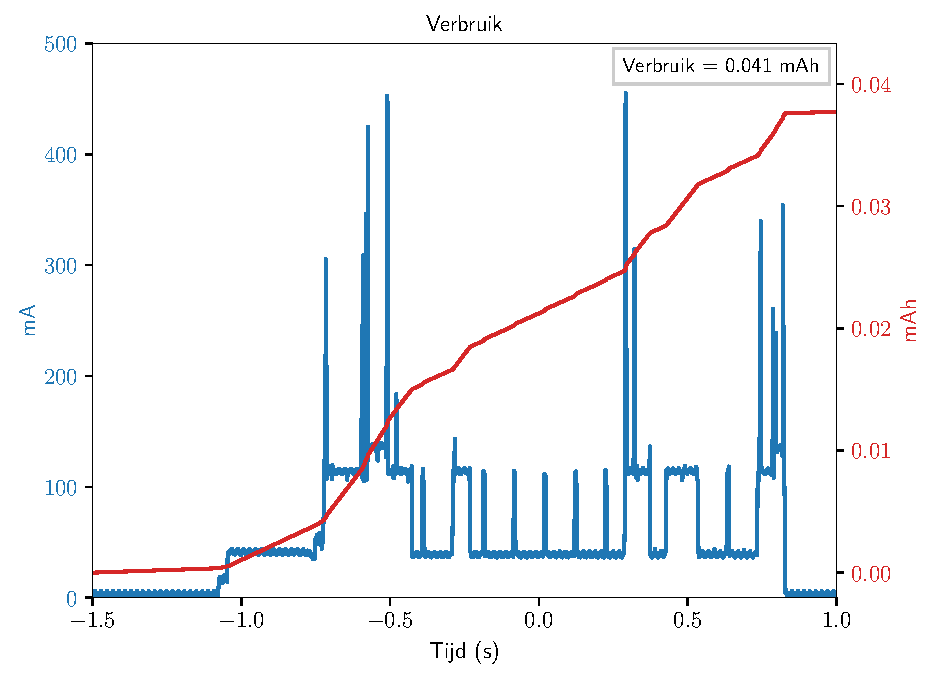
\includegraphics[width=1.0\linewidth]{wifi_pwr.pdf}
	\caption{Power consumption of one Wi-Fi transmission}
	\label{fig:wifi_pwr}
\end{figure}
In order to interpret the current consumption, the used charge is displayed in [mAh]. This results in 0.041 mAh of charge that is used in order to transmit the sensor data once. With this knowledge, we can calculate the amount of Wi-Fi transmissions that are possible with the 6400 mAh battery:

\begin{gather*}
	\frac{6400}{0.041} \approx 156097 \text{transmissions}
\end{gather*}

If there are 6 transmissions per hour and the system is active for 7 hours a day, this leads to a battery life off 3716 days.  However, this calculation only accounts for the Wi-Fi transmission, other power consumption such as stand-by power, CPU power and sensor power are not accounted for in this calculation. 

\section{Software design}
\paragraph{Functionality}
\begin{itemize}
	\item Pull sensors from sleep state every 10 minutes and read sensor values
	\item Send sensor data to server, over Wi-Fi
	\item Perform periodic synchronisations to get time information
	\item Use time information to disable power to sensors and put CPU in deepsleep during the night
\end{itemize}
\paragraph{Overview}
The software is based on a number of states these states are: NTPsync, checktime, nightsleep, wakefromnightsleep, wakesensors, readsensors, senddata and sleep. An overview of the complete software and the transitions between the states is illustrated in figure~\ref{fig:statediagram}. The states are discussed further below. 
\begin{figure}[!ht]
	\centering
	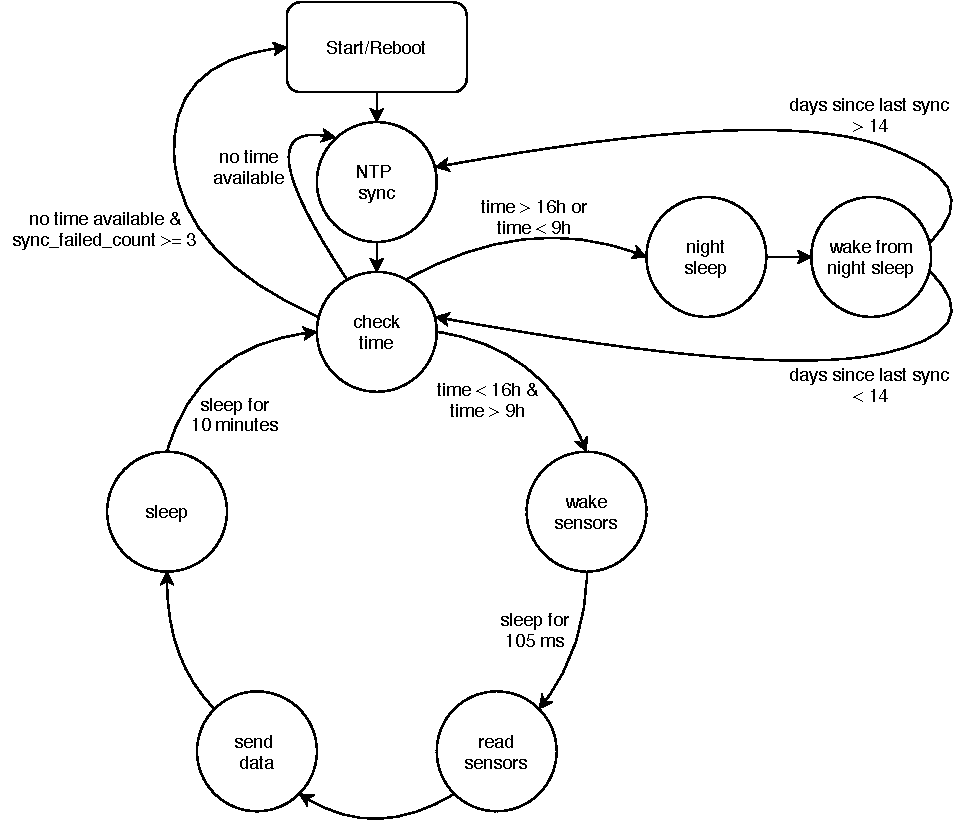
\includegraphics[width=1\linewidth]{statendiagram.pdf}
	\caption{State diagram}
	\label{fig:statediagram}
\end{figure}
\paragraph{NTP-sync}
In this state an NTP synchronisation is performed. This provides time information which is stored in the RTC memory and maintained by the RTC clock. The time information allows the system to know when it is night time. During the night the sensors can be disabled, using the load switches, and the microcontroller can go in to deepsleep until the morning. This way the sensors only receive power between 9 AM and 4 PM. 

\paragraph{Check time}
This state has two functionalities. Firstly the current time of day is retrieved from the RTC clock. If this time info is not available, the NTP synchronisation was not successful. When this is the case the microcontroller goes in to deepsleep for five minutes and the next state will be the NTP sync to retry the synchronisation. If the synchronisation fails three times, the system is rebooted. Next to this, when the synchronisation was successful, the time information will be available. This time information is then used to check the current time. If the time is between 9 AM and 4 PM the system remains active, thus the next state is set to wakesensors. If the time is after 4 PM and before 9 AM, the system has to go to sleep, thus the next state is set to nightsleep.

\paragraph{Night sleep}
This state is entered when it is past 4 PM and before 9 AM. During this time the sensors are disabled and the microcontroller goes in deepsleep. The sensors are disabled by raising the GPIO pins which control the load switches. When the GPIO pins are high, the load switches cut off the power to the sensors. Before entering deepsleep, the next state is set to wakefromnightsleep. During the night, no sensor data has to be collected and transmitted because the campus is closed. So by cutting off the power to the sensors and putting the microcontroller in deepsleep during the night the power consumption is drastically reduced. 

\paragraph{Wake from night sleep}
When the system wakes up at 9 AM, the power to the sensors has to be enabled. This is done by lowering the GPIO pins which control the load switches. Next to this, the system checks when the last synchronisation was performed. Because the RTC clock is derived from an internal RC oscillator with a frequency of \SI{150}{\kilo\hertz} and an accuracy of +/-5\% the clock time will drift away from the actual time. In order to prevent this, an NTP synchronisation has to be performed periodically. In order to retain an accurate clock, the synchronisation is performed every 14 days. Thus if the last synchronisation was performed 14 days ago, the next state is set to NTPsync. If the last synchronisation was more recent, the next state is set to checktime. 

\paragraph{Wake sensors}
In the wake sensors state, the sensors are taken out of their sleep state and put in active mode. When the sensors wake from their sleep state the sensor values can not be read immediately. A waiting period of 105 milliseconds is necessary in order to have stable sensor values. During these 105 milliseconds the sensors remain active but the microcontroller is put into deepsleep mode. Before entering deepsleep, the next state is set to readsensors. 

\paragraph{Read sensors}
In this state the sensor values are read out. Once the data is acquired, the sensors are put back in to their sleep state and the next state is set to senddata.

\paragraph{Send data}
In this state, the sensor data is transmitted to the python server which is running on a raspberry pi. Once the transmission is successful or the connection has timed-out the next state is set to sleep.

\paragraph{Sleep}
Once the sensor data has been transmitted to the server, the sleep state is entered. In this state, the microcontroller is put into deepsleep for 10 minutes. Before entering deepsleep, the next state is set to check time.


\section{Autonomy}

\subsection{Consumption sources}
In this section the different sources that consume power will be discussed.

\paragraph{Wi-Fi communication}
The system transmits the sensor data to the server over a Wi-Fi connection. This data transfer happens every 10 minutes. Because the sensors are disabled between 4 PM and 9 AM, no Wi-Fi connection is needed during that time. With a wake time of seven hours and 6 transmissions per day, this leads to 42 transmissions per day. A measurement of the typical power consumption for one Wi-Fi transmission is illustrates in figure~\ref{fig:wifipwr}.
\begin{figure}[!ht]
	\centering
	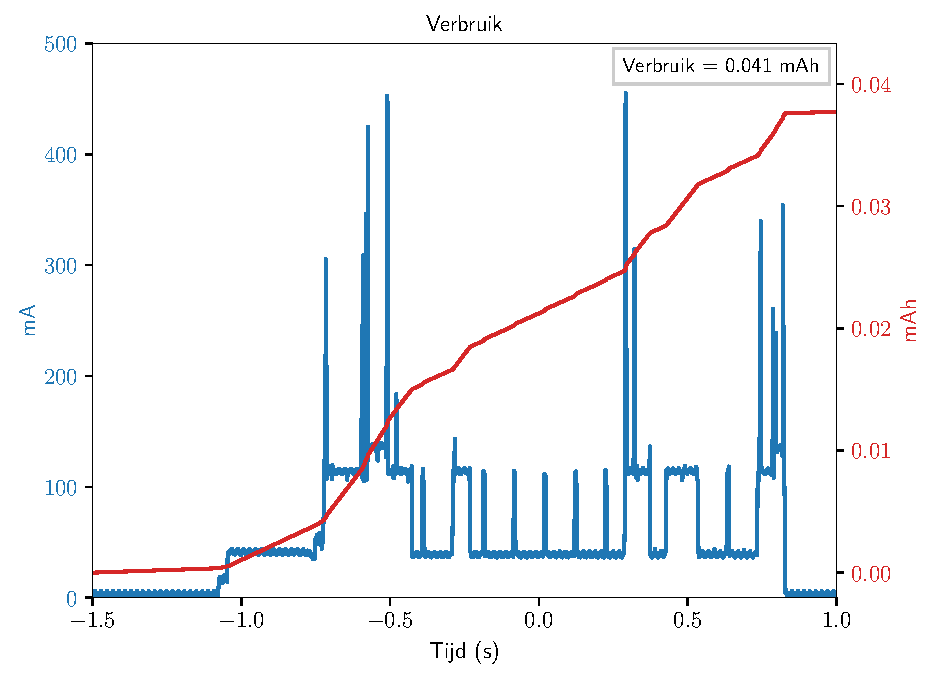
\includegraphics[width=1.0\linewidth]{wifi_pwr.pdf}
	\caption{Power consumption of one Wi-Fi transmission}
	\label{fig:wifipwr}
\end{figure}
The charge that is used for one transmission is 0.041 mAh. This leads to the following consumption per day:
\begin{gather*}
42 \cdot 0.041 = 1.722 \text{ mAh/day}
\end{gather*}

\paragraph{Sensors}
The sensors are read out every ten minutes. With a wake time of 7 hours\footnote{Only awake between 9 AM and 4 PM}, this leads to 42 sensor measurements per day. The power consumption to read out the sensors once is illustrates in figure~\ref{fig:sens_pwr}.

\begin{figure}[H]
	\centering
	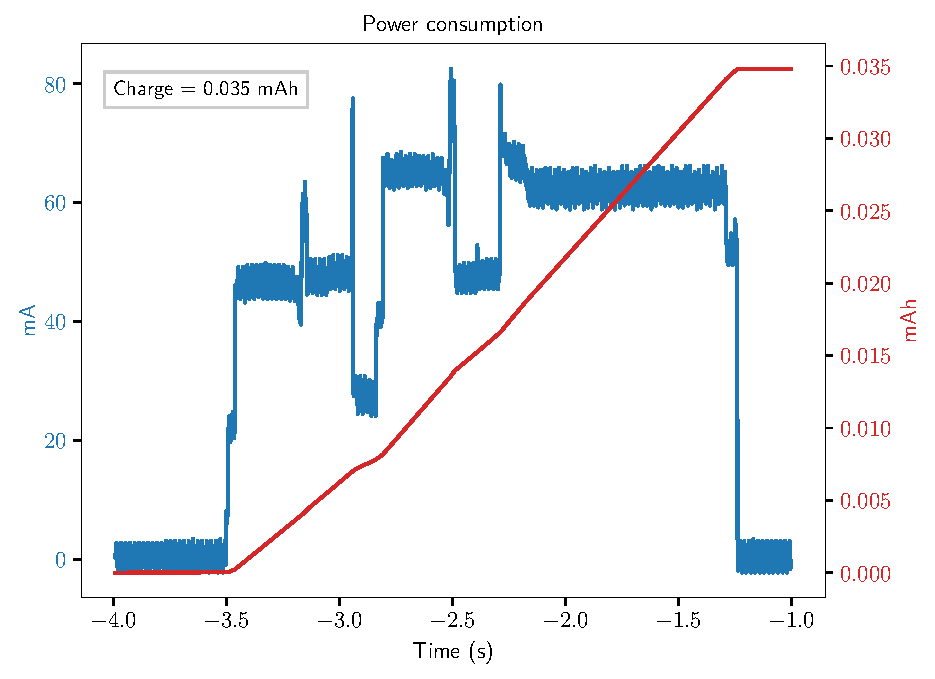
\includegraphics[width=1.0\linewidth]{sensor_pwr.pdf}
	\caption{Power consumption of one sensor measurement}
	\label{fig:sens_pwr}
\end{figure}

The charge that is used to read out the sensors once is 0.035 mAh. This leads to the following consumption per day:
\begin{gather*}
	42 \cdot 0.035 = 1.47\text{ mAh/day}
\end{gather*}

\paragraph{NTP synchronisation}
In order to synchronise the RTC clock an NTP synchronisation has to be performed periodically. This synchronisation is performed once every 14 days. The power consumption for one synchronisation is illustrates in figure~\ref{fig:ntp_pwr}.

\begin{figure}[H]
	\centering
	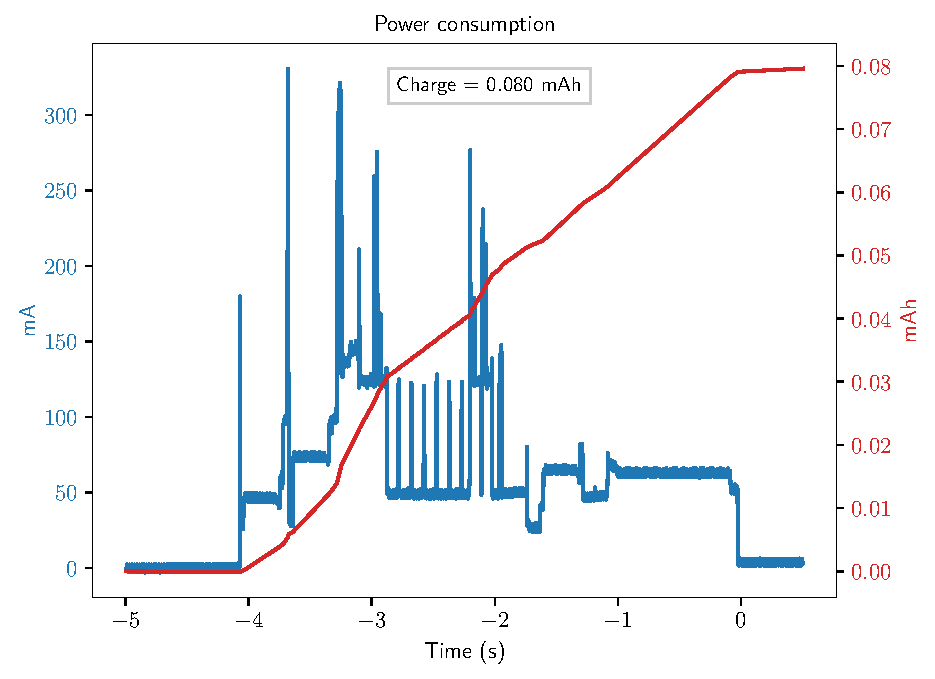
\includegraphics[width=1.0\linewidth]{sync_pwr.pdf}
	\caption{Power consumption of one NTP synchronisation}
	\label{fig:ntp_pwr}
\end{figure}

The charge that is used for one synchronisation is 0.08 mAh. However, this synchronisation only happens once very 14 days, this leads to the following consumption per day:
\begin{gather*}
	\frac{1}{14} \cdot 0.08 = 0.0057 \text{ mAh/day}
\end{gather*}

\paragraph{Standby daytime}\footnote{No measurement were performed to determine the stand-by power, this has two reasons. 1: the development board to test the software has an onboard LED which increases the power consumption so the gathered measurements wouldn't be representative. 2: to measure the power consumption a \SI{1}{\ohm} resistor was inserted between the power source and the development board. This resistor is used as a sense resistor but can not provide accurate \SI{}{\micro\ampere} measurements due to the noice that is introduced. }
Between 9 AM and 4 PM the system is 'active', this means that the sensors receive power. However when the sensors are not being read out they will be put in their respective sleep modes. The theoretical consumption that is gathered from the datasheets is listed below:
\begin{itemize}
	\item AMG8833 sleep mode: 0.2 mA
	\item CCS811 sleep mode: with $V_{dd}$ = \SI{1.8}{\volt}: 19 $\mu$A \\$\Rightarrow$ with $V_{dd}$ = \SI{3.3}{\volt}: $\frac{19}{1.8}\cdot 3.3 = 34.83 \text{ }\mu\text{A}$
	\item microphone: the power to the microphone is only enabled just before the measurement because of this the microphone has no stand-by/sleep consumption. 
\end{itemize}
Next to the consumption of the sensors, there is the sleep consumption of the microcontroller. If the microcontroller is not active, it is put in deepsleep. In deepsleep there is a consumption of 10 $\mu$A. Next to this consumption, two GPIO pins have to remain high during deepsleep: one to keep the CCS811 in sleep (nWake) and on to drive the load switch to disable the power to the microphone. The GPIO pins use an internal pull-up resistor of \SI{45}{\kilo\ohm} this leads to the following consumption for one GPIO pin: 
\begin{gather*}
	\frac{3.3 \text{V}}{45000\Omega} = 73.33 \text{ } \mu\text{A} 
\end{gather*}
For both GPIO pins this results in a consumption of 146.67 $\mu$A.
\\
For 7 hours a day the system is in active mode, this results in a charge consumption of:
\begin{gather*}
	7 \cdot (0.2 + 0.03483 + 0.01 + 0.1467) = 2.74\text{ mAh/day}
\end{gather*}

\paragraph{Standby nighttime}\footnote{No measurement were performed to determine the stand-by power, this has two reasons. 1: the development board to test the software has an onboard LED which increases the power consumption so the gathered measurements wouldn't be representative. 2: to measure the power consumption a \SI{1}{\ohm} resistor was inserted between the power source and the development board. This resistor is used as a sense resistor but can not provide accurate \SI{}{\micro\ampere} measurements due to the noice that is introduced. }
Between 4 PM and 9 AM the system goes in to sleep mode. In sleep mode no sensor measurements are performed and no data is transferred via Wi-Fi. To reduce the power, the power to the sensors is cut-off by using the load switches. The remaining stand-by/sleep consumption originates from the CPU consumption in deepsleep and the three GPIO pins that are kept high to drive the load switches. This leads to the following consumption:
\begin{gather*}
	10 \text{ }\mu\text{A} + 3\cdot 73.33\text{ }\mu\text{A} = 230\text{ }\mu\text{A}
\end{gather*}
The system remains in sleep mode for 17 hours a day this leads to the following consumption per day:
\begin{gather*}
	17 \cdot 230\text{ }\mu\text{A}= 3.91\text{ mAh}
\end{gather*}

\subsection{Total power consumption}
In the previous section all the different sources that consume power were discussed an overview is given in table~\ref{tab:pwr}.

\begin{table}[H]
	\centering
	\begin{tabular}{|l|l|}
	\hline
	\textit{\textbf{Source}} & \textbf{Charge per day {[}mAh/day{]}} \\ \hline
	Wi-Fi                    & 1.722 mAh/day                         \\ \hline
	Sensors                  & 1.47 mAh/day                          \\ \hline
	NTP sync                 & 0.0057 mAh/day                        \\ \hline
	Standby daytime          & 2.74 mAh/day                          \\ \hline
	Standby nighttime        & 3.91 mAh/day                          \\ \hline
	\rowcolor{Gray}
	Total                    & 9.85 mAh/day  						 \\ \hline
	\end{tabular}
	\captionsetup{justification=centering}
	\caption{Overview of the power consumption per day}
	\label{tab:pwr}
\end{table}

There are two Li-Ion cells that are used to power the system, they both have a capacity of 3200 mAh which results in a total capacity of 6400 mAh. This leads to the following battery life:
\begin{gather*}
	\frac{6400}{9.85}=649 \text{ days}
\end{gather*}


\section{DashBoard}
\paragraph{Functionality}
\begin{itemize}
	\item Recieve the data from the sensor
	\item Store the data in a database
	\item Display an overview with the avarages of every sensor
	\item Display the data from each sensor on a heatmap
\end{itemize}

\paragraph{Overview}
The intention of this dashboard is to display the data that the different sensors on all the devices in the cafeteria generate.
It gives an overview of what's happening in the cafeteria in an airquality, temperature and sound perspective. 
The infrared camera data which is an 8 by 8 pixel picture is drawn on a heatmap. 
This gives a nice overview of the busy and the less busy area's in the cafeteria.  

\subsection{Backend}
The backend is what runs on our server, in this project a raspberry pi was chosen as it's an easy to use and small computer
 that can easily be set up to be used as a webserver that hostes our dashboard and the database that is used to store the data.

\paragraph{Recieve data}
To recieve the data a python script (WiFi.py) is used that listens to the 8091 port, this is the port that the device sends his payload to.
The protocol that is used to send data from the device to the raspberry pi is TCP. A more in depth explanation can be found in \nameref{wifiCon}.

\paragraph{Store data}
The recieved data is stored in a mysql database, this is also implemented in the WiFi.py script that is used to recieve the data.
To use the database in the python script a mysql.connector is used.
The database uses 3 tables: 
\begin{itemize}
	\item location: this table is used to store the location of the sensor. It has an x-, y-coordinate and the location id.
	\item sensor: this table stores the sensor id  and has the location id as a foreign key.
	\item readings: This is the table that stores all the sensor data with the date and time that it was recieved. 
					All the data that isn't an array is stored as a float, the arrays with the 64 pixels from the infrared camera are stored as a json string.
					The two other columms in this table are the reading id and the sensor id.  
\end{itemize}
A visual representation of the database descript above can be seen in figure~\ref{fig:db_des}.

\begin{figure}[H]
	\centering
	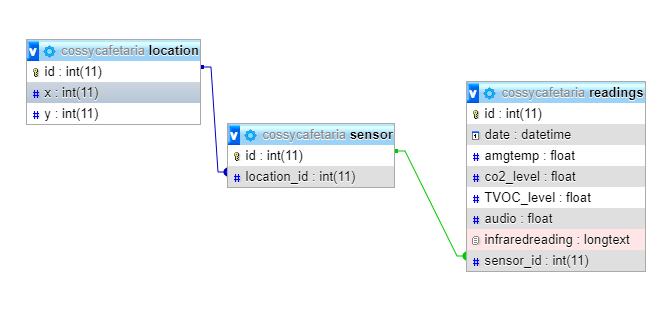
\includegraphics[width=1.0\linewidth]{databaseDesign.png}
	\caption{Visual represntation of the database}
	\label{fig:db_des}
\end{figure}

\paragraph{Serve data to dashboard}
A php script is used to serve the data to the frontend of the dashboard. This php script is called database.php. 
It's a simple script that connects to the database on the raspberry pi and gets the last recieved data from all the different devices.
Then all this data is encoded as json and passed on to the website that is used as dashboard. 

\subsection{Frontend}


\section{Financial estimate}
Kostprijs van het project opstellen.

\section{Validation and measurements}
Hier moeten we aantonen of dat alles werkt. Of eventuele fouten verklaren.

% bibliografie toevoegen
\newpage
\bibliography{bibliography}	

%----------------------------------------------------------------------------------------
%	Bijlagen
%----------------------------------------------------------------------------------------
\newpage
\appendix
\section{MainPCB schematic}\label{app:mainpcb_schematic}
%\begin{figure}[H]
%	\centering
%	\includegraphics[width=1\linewidth]{MainPCB_schematic.pdf}
%\end{figure}
\includepdf[pages=-]{fig/MainPCB_schematic.pdf}

\newpage

\end{document}